\newgeometry{margin=0.75in}
\textbf{This text is licensed under a Creative Commons Attribution-Share Alike 3.0 United States License.}\\

To view a copy of this license, visit \href{http://creativecommons.org/licenses/by-sa/3.0/us/}{http://creativecommons.org/licenses/by-sa/3.0/us/} or send a letter to Creative Commons, 171 Second Street, Suite 300, San Francisco, California, 94105, USA\\

You are \textbf{free}:\\
\hspace*{0.25in} \textbf{to Share} -- to copy, distribute, display, and perform the work\\
\hspace*{0.25in} \textbf{to Remix} -- to make derivative works\\

Under the following conditions:\\
\hspace*{0.25in} \textbf{Attribution.}  You must attribute the work in the manner specified by the author or licensor (but not in any way that suggests that they endorse you or your use of the work).\\
\hspace*{0.25in} \textbf{Share Alike.}  If you alter, transform, or build upon this work, you may distribute the resulting work only under the same, similar, or a compatible license.\\

With the understanding of the following:\\
\hspace*{0.25in} \textbf{Waiver.}  Any of the above conditions can be waived if you get permission from the copyright holder.\\
\hspace*{0.25in} \textbf{Other Rights.}  In no way are any of the following rights affected by the license:
\begin{itemize}
\item Your fair dealing or fair use rights
\item Apart from the remix rights granted under this license, the authors' moral rights
\item Rights other persons may have either in the work itself or in how the work is used, such as publicity or privacy rights
\item Notice --- For any reuse or distribution, you must make clear to others the license terms of this work.  The best way to do this is with a link to the following web page: \href{http://creativecommons.org/licenses/by-sa/3.0/us/}{http://creativecommons.org/licenses/by-sa/3.0/us/}
\end{itemize}

\paragraph{Attributions} This book benefited tremendously from others who went before and freely shared their creative work.  The following is a short list of those whom we have to thank for their work and their generosity in contributing to the free and open sharing of knowledge.
\begin{itemize}
\item David Lippman, author of \textit{Math in Society}.  This book uses sections derived from his chapters on Finance, Growth Models, and Statistics.  He also administers MyOpenMath, the free online homework portal to which the problems in this text were added.
\item The developers of \href{onlinestatbook.com}{onlinestatbook.com}.
\item OpenStax College (their book \textit{Introductory Statistics} was used as a reference)

OpenStax College, \textit{Introductory Statistics}. OpenStax College. 19 September 2013. <http://cnx.org/content/col11562/latest/>
\item The authors of \href{https://www.openintro.org/stat/?stat_book=os}{OpenIntro Statistics}, which was also used as a reference.
\item The Saylor Foundation Statistics Textbook: http://www.saylor.org/site/textbooks/Introductory$\%$20Statistics.pdf
\end{itemize}

\paragraph{Thanks} The following is a short list of those whom we wish to thank for their help and support with this project.
\begin{itemize}
\item The President's office at Frederick Community College, for providing a grant to write the first chapters.
\item Gary Hull, who in his tenure as department chair gave us his full support and gave us the impetus to start the project, and generously shared his notes for MA 103.
\item The entire FCC math department, who provided untold support and encouragement, as well as aid in reviewing and editing the text.
\end{itemize}

\vfill
\pagebreak

\subsection{Example Videos}
\parbox{0.75\textwidth}{Every example in the book has an accompanying video; to view the video, click on the title of the example or the example number in the margin.}
\begin{center}
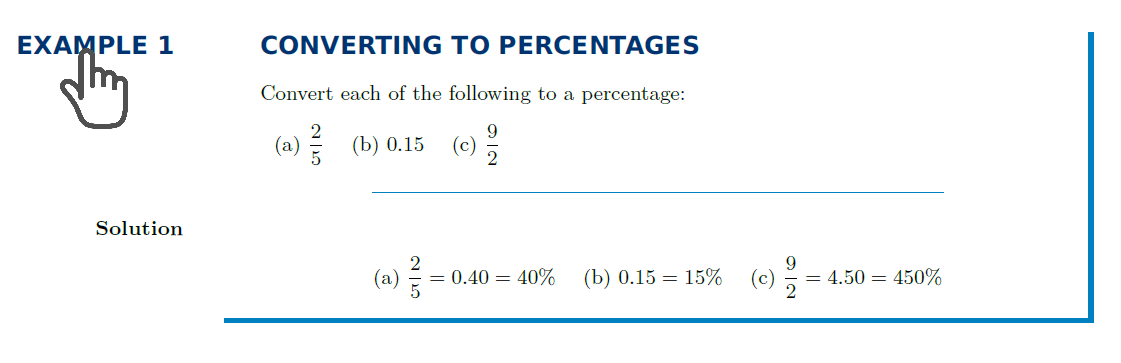
\includegraphics[width=0.75\textwidth]{examplehowto}
\end{center}

\subsection{Try It}
\parbox{0.75\textwidth}{Many examples are followed by Try It examples, which can be used for extra practice.  Clicking on the words Try It in the margin will open a web page where students can enter their answers and check them.}
\begin{center}

\includegraphics[width=0.75\textwidth]{tryithowto}
\end{center}

\subsection{Free Online Homework}
\parbox{0.75\textwidth}{Versatile Math includes free online homework, provided through MyOpenMath.}
\begin{center}
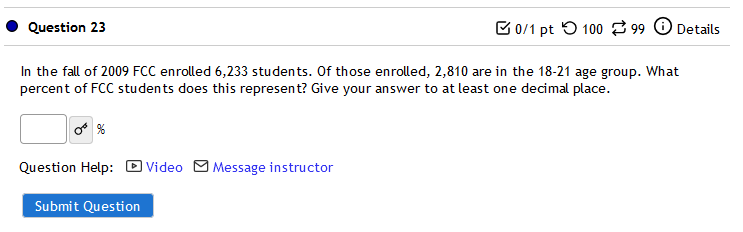
\includegraphics[width=0.75\textwidth]{homeworkscreenshot}
\end{center}
\vfill
\pagebreak

\subsection{What's New in the 2nd Edition}
\paragraph{Chapter 1}
\begin{itemize}
\item A new introduction section was added, describing many of the initial concepts used in the chapter.
\item The income tax section was moved to the end of the chapter and updated to reflect changes to the U.S. tax code (including 2020 tax brackets); the discussion of deductions and credits was expanded with new graphics.
\item The discussion of inflation was removed, since it made the section on simple and compound interest too long.
\item New examples were added to the retirement section, showing how to plan fully for retirement.
\item A description of the use of Excel and the TVM solver on TI graphing calculators was added to several sections. 
\end{itemize}

\paragraph{Chapter 2}
\begin{itemize}
\item A new section on quadratic models was added.
\item A discussion on using a calculator to do regression with each type of model was added.
\item In the section on exponential models, the discussion was condensed by eliminating models of the form $P_t = P_0e^{kt}$ and Newton's law of cooling.
\end{itemize}

\paragraph{Chapter 3}
\begin{itemize}
\item The entire chapter was reordered:
\begin{itemize}
\item The old first section was split, expanding the discussion of gathering data and graphing it into two separate sections.
\item The discussion of sampling methods was expanded, and new graphs were introduced, including dot plots and scatterplots.
\item The next two sections (measures of center and measures of spread) were merged into a single section on describing data with statistics.
\item A new section was added on the use of linear regression.
\end{itemize}
\end{itemize}

\paragraph{Chapters 4--7} These remained mostly unchanged.

\paragraph{Chapter 8} A new chapter on Graph Theory was added, with all-new videos and homework.

\paragraph{Chapter R} A short review of some algebra concepts used throughout the book was added.

%\restoregeometry




















